\chapter{Arhitektura i dizajn sustava}
		
		\textbf{\textit{dio 1. revizije}}\\

		\textit{ Potrebno je opisati stil arhitekture te identificirati: podsustave, preslikavanje na radnu platformu, spremišta podataka, mrežne protokole, globalni upravljački tok i sklopovsko-programske zahtjeve. Po točkama razraditi i popratiti odgovarajućim skicama:}
	\begin{itemize}
		\item 	\textit{izbor arhitekture temeljem principa oblikovanja pokazanih na predavanjima (objasniti zašto ste baš odabrali takvu arhitekturu)}
		\item 	\textit{organizaciju sustava s najviše razine apstrakcije (npr. klijent-poslužitelj, baza podataka, datotečni sustav, grafičko sučelje)}
		\item 	\textit{organizaciju aplikacije (npr. slojevi frontend i backend, MVC arhitektura) }		
	\end{itemize}
	
	
	
	
	
	\begin{packed_item}
	\item \textbf{Proces odabira arhitekture}
	\end{packed_item}
		U našem je zadatku cilj web aplikacije olakšati darivateljima krvi i Crvenom Križu cijeli proces darivanja krvi: od organiziranja akcija do pronalaženja istih i rezerviranja termina. Specifikacijom dionika i definiranjem funkcionalnih zahtjeva zaključili smo kako naša aplikacija mora imati tri razine: razinu baze podataka, razinu web-aplikacije i razinu klijenta. Tako navedenim razinama korespondiraju tri sloja: sloj pristupa podacima, sloj aplikacijske logike i sloj korisničkog sučelja. Razmatrajući potrebna svojstva, poput smanjivanja nepotrebnih međuovisnosti između modula radi jednostavnosti pri budućim promjenama, hijerarhijske organizacije razina koja omogućava pristup viših razina nižima preko programskog sučelja i grupiranje dijelova programa koji pristupaju i mijenjaju iste podatke te procedura koje se izvode slijedno radi lakšeg snalaženja, odabrali smo višeslojnu arhitekturu temeljenu na klijent-poslužitelj odnosu, najsličniju MVC stilu arhitekture.
	
	\begin{packed_item}
	\item \textbf{Višeslojna arhitektura i MVC stil}
	\end{packed_item}
		Odnos klijent-poslužitelj opisuje međusobni odnos programa koji sudjeluju u aplikaciji, to jest njihovo funkcioniranje prije, tijekom i po završetku komunikacije klijenta i poslužitelja. Aplikacija sadrži tri osnovna sloja: 
	
	\begin{itemize}
	\item[] \begin{packed_enum}
		\item \underbar{Klijentsku komponentu} - sloj s korisničkim sučeljem, predstavljena web preglednikom, služi kao sučelje između klijenta i poslužitelja, omogućava klijentu slanje HTTP zahtjeva i primanje HTTP odgovora, prevoditelj koji web stranicu pisanu u kodu prikazuje u klijentu razumljivom obliku
		\item \underbar{Poslužiteljsku komponentu} - sloj aplikacijske logike, predstavlja web poslužitelj, centar za razmjenu informacija i pružanje usluga, služi za pohranu, obradu i dostavu web stranica klijentu, pokreće web aplikaciju i prosljeđuje joj klijentove zahtjeve, po potrebi pristupa bazi podataka i vraća klijentu odgovor vidljiv u web pregledniku
		\item \underbar{Baza podataka} - sloj za pohranu podataka
	
	\end{packed_enum}
	\end{itemize}
	
	\begin{figure}[H]
		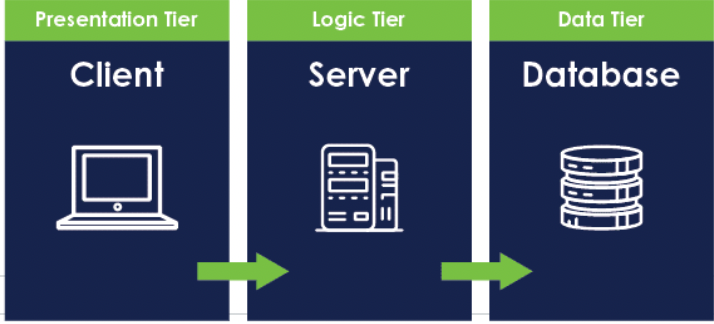
\includegraphics[scale=0.4]{slike/troslojnaArhitektura.png} %veličina slike u odnosu na originalnu datoteku i pozicija slike
		\centering
		\caption{Troslojna arhitektura}
		\label{fig:troslojnaArhitektura}
	\end{figure}
	
	
		Prednost klijent-server arhitekture je mogućnost odvojenog oblikovanja slojeva, što također omogućava “separation of concerns”, to jest svaki sloj brine samo za svoju zadaću i ne brine o funkcionalnostima drugih slojeva, a njihova se međuovisnost ostvaruje komunikacijom pomoću sučelja. 
		Ovako razrađenoj arhitekturi, najsličniji je Model-View-Controller stil. Osnovna je karakteristika ovog stila razdvajanje briga nezavisnim razvojem pojedinih dijelova aplikacije, što omogućuje jednostavnije i učinkovitije testiranje i izmjene dijelova sustava radi njihove dorade te skalabilnost i fleksibilnost cijele aplikacije razvijene na ovakvom principu. Korisničko sučelje je odvojeno od ostatka sustava, a povezanost elemenata se ostvaruje kroz tri sloja: sloja “View” na klijentskoj strani, te slojeva “Model” i “Controller” na poslužiteljskoj strani.
	\begin{packed_item}
		

	\item[] \begin{packed_enum}
		\item \textit{Model (model)} - predstavlja podatke i logiku vezanu za njih, služi za oblikovanje podataka i prilagodbu komunikaciji s bazom
		\item \textit{View (pogled)} - komunikacija s korisnikom i prikaz podataka koje je dobio od upravitelja
		\item \textit{Controller (upravitelj)} - povezuje modele i poglede, na temelju primljenih korisničkih zahtjeva i podataka izvršava potrebne funkcije i formira odgovore
		
	\end{packed_enum}
	\end{packed_item}
	
	\begin{figure}[H]
		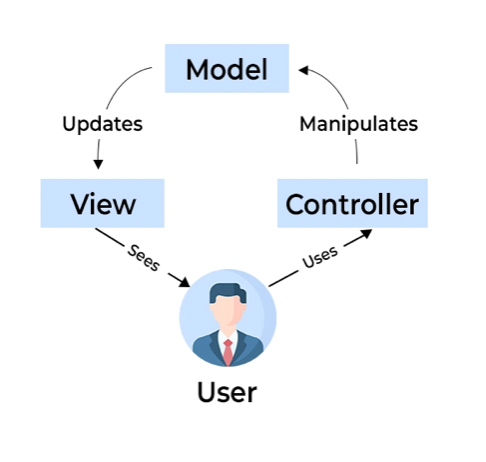
\includegraphics[scale=0.4]{slike/MVC.png} %veličina slike u odnosu na originalnu datoteku i pozicija slike
		\centering
		\caption{MVC stil arhitekture}
		\label{fig:mvc}
	\end{figure}
	
	
		Web aplikacija je podijeljena na front-end i back-end.
		Front-end čini prezentacijski dio aplikacije, to jest ono što korisnik vidi u web pregledniku. Za izradu aplikacije na klijentskoj strani odabrali smo radni okvir React, koji je zasnovan na JavaScriptu i pruža učinkovit razvoj korisničkog sučelja koristeći već gotove web komponente.
		Back-end čini dio sustava u kojem se obrađuju korisnički zahtjevi i vrše potrebne akcije, to jest poslužiteljska strana klijent-server arhitekture. Za njegovu smo izradu odabrali programski jezik Python i radni okvir FastAPI.
		I za razvoj klijentske i za razvoj poslužiteljske strane odabrali smo Visual Studio Code kao radno okruženje.
		
	

				
		\section{Baza podataka}
			
			\textbf{\textit{dio 1. revizije}}\\
			
		\textit{Potrebno je opisati koju vrstu i implementaciju baze podataka ste odabrali, glavne komponente od kojih se sastoji i slično.}
		
			\subsection{Opis tablica}
			

				\textit{Svaku tablicu je potrebno opisati po zadanom predlošku. Lijevo se nalazi točno ime varijable u bazi podataka, u sredini se nalazi tip podataka, a desno se nalazi opis varijable. Svjetlozelenom bojom označite primarni ključ. Svjetlo plavom označite strani ključ}
				
				
				\begin{longtblr}[
					label=none,
					entry=none
					]{
						width = \textwidth,
						colspec={|X[6,l]|X[6, l]|X[20, l]|}, 
						rowhead = 1,
					} %definicija širine tablice, širine stupaca, poravnanje i broja redaka naslova tablice
					\hline \SetCell[c=3]{c}{\textbf{korisnik - ime tablice}}	 \\ \hline[3pt]
					\SetCell{LightGreen}IDKorisnik & INT	&  	Lorem ipsum dolor sit amet, consectetur adipiscing elit, sed do eiusmod  	\\ \hline
					korisnickoIme	& VARCHAR &   	\\ \hline 
					email & VARCHAR &   \\ \hline 
					ime & VARCHAR	&  		\\ \hline 
					\SetCell{LightBlue} primjer	& VARCHAR &   	\\ \hline 
				\end{longtblr}
				
				
			
			\subsection{Dijagram baze podataka}
				\textit{ U ovom potpoglavlju potrebno je umetnuti dijagram baze podataka. Primarni i strani ključevi moraju biti označeni, a tablice povezane. Bazu podataka je potrebno normalizirati. Podsjetite se kolegija "Baze podataka".}
			
			\eject
			
			
		\section{Dijagram razreda}
		
			\textit{Potrebno je priložiti dijagram razreda s pripadajućim opisom. Zbog preglednosti je moguće dijagram razlomiti na više njih, ali moraju biti grupirani prema sličnim razinama apstrakcije i srodnim funkcionalnostima.}\\
			
			\textbf{\textit{dio 1. revizije}}\\
			
			\textit{Prilikom prve predaje projekta, potrebno je priložiti potpuno razrađen dijagram razreda vezan uz \textbf{generičku funkcionalnost} sustava. Ostale funkcionalnosti trebaju biti idejno razrađene u dijagramu sa sljedećim komponentama: nazivi razreda, nazivi metoda i vrste pristupa metodama (npr. javni, zaštićeni), nazivi atributa razreda, veze i odnosi između razreda.}\\
			
			\textbf{\textit{dio 2. revizije}}\\			
			
			\textit{Prilikom druge predaje projekta dijagram razreda i opisi moraju odgovarati stvarnom stanju implementacije}
			
			
			
			\eject
		
		\section{Dijagram stanja}
			
			
			\textbf{\textit{dio 2. revizije}}\\
			
			\textit{Potrebno je priložiti dijagram stanja i opisati ga. Dovoljan je jedan dijagram stanja koji prikazuje \textbf{značajan dio funkcionalnosti} sustava. Na primjer, stanja korisničkog sučelja i tijek korištenja neke ključne funkcionalnosti jesu značajan dio sustava, a registracija i prijava nisu. }
			
			
			\eject 
		
		\section{Dijagram aktivnosti}
			
			\textbf{\textit{dio 2. revizije}}\\
			
			 \textit{Potrebno je priložiti dijagram aktivnosti s pripadajućim opisom. Dijagram aktivnosti treba prikazivati značajan dio sustava.}
			
			\eject
		\section{Dijagram komponenti}
		
			\textbf{\textit{dio 2. revizije}}\\
		
			 \textit{Potrebno je priložiti dijagram komponenti s pripadajućim opisom. Dijagram komponenti treba prikazivati strukturu cijele aplikacije.}